% !TEX encoding = UTF-8
% !TEX TS-program = pdflatex
% !TEX root = ../tesi.tex

%**************************************************************
\chapter{Introduzione}
\label{cap:introduzione}
%**************************************************************
\section{L'azienda}

\company{} è un'azienda italiana, di piccole dimensioni, che da 25 anni sviluppa soluzioni software per altre aziende e privati.\\
L'azienda lavora su 5 diversi macro-progetti, uno dei quali è Engagent, la chatbot professionale oggetto dei miei due mesi di stage.\\
Dal 2013, PAT è entrata a far parte di Zucchetti Group.
\begin{figure}[H]
    \centering
    
\includegraphics[width=0.3\columnwidth]{logo-pat.png} 
    \caption{logo \company{}}
    \label{logo:company}
\end{figure}

\subsection{Prodotti e servizi}
L'azienda offre ai suoi clienti l'automatizzazione dei processi e il miglioramento dell'\textit{user experience} dei loro prodotti.
PAT concretizza quesi obiettivi attraverso i seguenti prodotti:
\begin{itemize}
    \item Engagent: chatbot semi-automatizzata per uso professionale, l'unico prodotto di \company{} con cui sono entrato in cotatto; 
    \item Helpdesk;
    \item Infinite: \textit{CRM} software orientato alla relazione tra cliente e azienda;
    \item Brain \textit{Interactive}: piattaforma per governare dei servizi personalizzati attraverso dei diagrammi di flusso; 
    \item Teammee: piattaforma per la comunicazione tra i dipendenti in un'azienda, usando la logica dei social networks;
\end{itemize}

\subsubsection{Engagent}

Engagent è una chatbot orientata al business, con un agente virtuale integrato. In \textit{backend}, un motore semantico permette di capire cosa sta chiedendo l'utente e trovare la risposta più coerente. Se la domanda è troppo complessa, il motore semantico estrate la categoria della domanda e la reinderizza all'operatore adeguato.
\begin{figure}[H]
    \centering
    
\includegraphics[width=0.3\columnwidth]{logo_engagent.png} 
    \caption{logo Engagent}
    \label{logo:company}
\end{figure}
\subsection{Organizzazione e Metodo di lavoro}
L'azienda è divisa in più gruppi di lavoro, uno per ogni macro-progetto, oltre alla segreteria e direzione.\\
Ogni team è separato dagli altri, anche se la collaborazione tra le parti è necessaria.\\
Tutti i team di sviluppo in \company{} seguono una metodologia Agile. Questa fa parte delle metodologie iterative, caratterizzata da brevi iterazioni (o sprint, di circa 3-4 settimane) seguite dalla \textit{review} del lavoro svolto. Il focus principale si trova nel cliente: ci deve essere una interazione costante per capire quali sono le \textit{feature} più importanti, che hanno precedenza sulle altre.\\
Il team a cui ho preso parte applica questa metodologia. Il contatto con il cliente è frequente, che sia manutenzione o nuove \textit{features} da implementare. La piccola dimensione del team e le riunioni giornaliere permettono una buona collaborazione. Il team è gestito da un responsabile che organizza le riunioni e comunica con il manager dell'azienda.\\
Per quanto mi rigurarda, ho adottato senza difficoltà queste metodologie, perché molto simili a quelle utilizzate durante il progetto di ingegneria del software.
\begin{figure}[H]
    \centering
    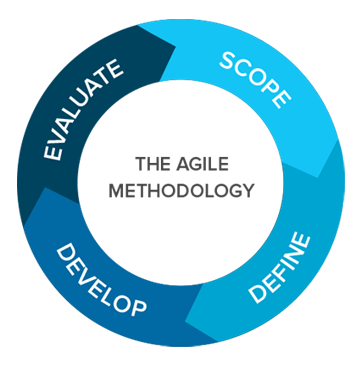
\includegraphics[width=0.3\columnwidth]{agile.png} 
    \caption{Agile}
    \label{logo:company}
\end{figure}

%**************************************************************
\section{Strumenti e Tecnologie}
Questa sezione descrive, ad alto livello, le tecnologie utilizzate durante lo stage.
\subsection{Ambiente di lavoro}
L'ambiente di lavoro utilizzato è Windows 10, assieme al pacchetto office per la maggior parte delle attività.\\
I team di sviluppo hanno libera scelta sugli editor. Per la codifica e la stesura dei docuemnti, ho scelto Visual studio. Per la creazione di diagrammi UML, ho utilizzato Astah UML.\\
Ogni sviluppatore ha a disposizione un PC fisso e un portatile per le riunioni.

\subsection{Linguaggi di programmazione}
I linguaggi di programazione che ho utilizzato sono:
\begin{itemize}
    \item \textbf{Python:} per implementare l'applicazione;
    \item \textbf{Shell:} per la creazione di script per automatizzare alcuni task:
    \begin{itemize}
        \item esecuzione del programma tramite linea di comando;
        \item pulizia della cache del programma;
        \item pulizia dei file di output del programma.
    \end{itemize}
\end{itemize}

%**************************************************************
\section{Organizzazione del testo}

\begin{description}
    \item[{\hyperref[cap:introduzione]{Il primo capitolo}}] contiene una panoramica dell' azienda e le tecnologie utilizzate \company{};

    \item[{\hyperref[cap:descrizione-stage]{Il secondo capitolo}}] contiene la pianificazione progetto; 
    
    \item[{\hyperref[cap:analisi-requisiti]{Il terzo capitolo}}] approfondisce nel dettaglio i requisiti del progetto, descrivendo il processo di analisi che ha portato alla loro stesura;
    
    \item[{\hyperref[cap:progettazione-codifica]{Il quarto capitolo}}] approfondisce l'architettura del software sviluppato, con il supporto di esempi specifici e schemi ad alto livello;
        
    \item[{\hyperref[cap:conclusioni]{Il quinto capitolo}}] contiene il resoconto del progetto e considerazioni personali sullo stage. 
\end{description}